% ============================================================
% Hybrid-Enhanced ATSC Paper
% Compile: pdflatex main -> bibtex main -> pdflatex main (x2)
% ============================================================
\documentclass[conference]{IEEEtran}
\IEEEoverridecommandlockouts

\usepackage{cite}
\usepackage{amsmath,amssymb,amsfonts}
\usepackage{graphicx}
\usepackage{textcomp}
\usepackage{xcolor}
\usepackage{booktabs}
\usepackage{multirow}
\usepackage{array}
\usepackage{balance}
\usepackage{url}

\def\BibTeX{{\rm B\kern-.05em{\sc i\kern-.025em b}\kern-.08em
    T\kern-.1667em\lower.7ex\hbox{E}\kern-.125emX}}

\begin{document}

\title{Hybrid-Enhanced Deep Reinforcement Learning for Adaptive Traffic Signal Control at an Isolated Four-Way Intersection}

\author{
\IEEEauthorblockN{[Author Names Omitted for Review]}
\IEEEauthorblockA{[Affiliation Omitted for Review]}
}

\maketitle

\begin{abstract}
Adaptive traffic signal control remains one of the most practical
single-intersection applications of reinforcement learning, yet
performance still depends heavily on how the controller represents
traffic structure and handles phase switching. This paper revisits a
movement-based four-action adaptive traffic signal control benchmark
and introduces a new controller, termed
\emph{Hybrid-Enhanced Pri-Hyper DDQN}. The proposed method combines
the most effective ideas from two strong deep baselines: the
priority-replay, Double-DQN-oriented learning strategy of Pri-DDQN
and the temporal relational state modelling of MA-SAC. The resulting
architecture integrates prioritized double dueling Q-learning, a
temporal hypergraph encoder over movement groups, a pressure-aware
action prior, and conservative switch selection to reduce unnecessary
yellow-loss penalties. Experiments are conducted on the same
stochastic four-way intersection simulator used for the repository
benchmarks, with identical actions, reward design, horizon, and
evaluation seeds. The proposed controller achieves the best traffic
efficiency among all evaluated methods, reducing average queue length
to 0.863, average waiting time to 19.146~s, and total delay to
24\,864.33 vehicle-seconds, outperforming the existing Pri-DDQN and
MA-SAC baselines on these operational metrics. Pri-DDQN retains the
best scalar benchmark reward, but the Hybrid-Enhanced method delivers
the most robust traffic-serving behaviour overall. These results show
that combining value-based deep RL with structured relational traffic
encoding and domain-aware action shaping is a strong direction for
isolated intersection control.
\end{abstract}

\begin{IEEEkeywords}
adaptive traffic signal control, reinforcement learning, Double DQN,
hypergraph encoder, prioritized replay, traffic signal control,
isolated intersection, deep reinforcement learning
\end{IEEEkeywords}

\section{Introduction}
Urban congestion is felt most sharply at signalised intersections,
where local control decisions accumulate into measurable delays,
queues, fuel losses, and driver frustration. Fixed-time plans remain
widely used because they are predictable and easy to deploy, but
their weakness is equally well known: they cannot react to the
short-term imbalance and stochasticity of real traffic arrivals.
Adaptive traffic signal control (ATSC) therefore remains an active
area of research, especially for isolated intersections where better
control can be achieved without the full complexity of large network
coordination.

Reinforcement learning (RL) is a natural fit for ATSC because it
allows a controller to improve directly from repeated interaction
with traffic dynamics. Classical tabular methods established the
basic feasibility of this paradigm for isolated intersections
\cite{ElTantawy2014DesignORH,Touhbi2017AdaptiveTSM}, while later
deep RL methods extended it to richer state descriptions and more
complex phasing choices \cite{Haydari2020DeepRLC,Gu2020DoubleDQD}.
Among recent single-intersection approaches, Pri-DDQN
\cite{Zheng2024PriDDQNLAG} is particularly appealing because it
stabilizes value learning through Double DQN, prioritized replay,
power-function exploration decay, and state/reward-aware weighting.
At the same time, the MA-SAC framework
\cite{Wang2024TowardMRP}, though originally designed for
multi-intersection coordination, highlights a complementary strength:
traffic states are relational and temporal, not merely flat vectors.

These two observations motivate the present work. In our benchmark,
Pri-DDQN attains the strongest overall scalar reward, while MA-SAC
demonstrates the usefulness of structured state modelling.
However, neither method fully combines both strengths. Pri-DDQN is
strong in optimization strategy but relatively flat in state
representation; MA-SAC is strong in representation but less well
aligned with small discrete action ranking under switching
penalties. We therefore propose a new method,
\emph{Hybrid-Enhanced Pri-Hyper DDQN}, which explicitly fuses:

\begin{itemize}
\item prioritized double dueling Q-learning,
\item temporal hypergraph encoding of movement groups,
\item a pressure-aware action prior, and
\item conservative switch filtering to suppress weak phase changes.
\end{itemize}

The paper focuses on the movement-based four-action benchmark rather
than the simpler two-action setting because the four-action problem
is where controller design becomes genuinely interesting. It asks the
agent to allocate service not only between north--south and
east--west axes, but also between straight-through and protected
left/U-turn movements. This creates a more realistic control problem
with stronger trade-offs between throughput, fairness, and switching
cost.

The main contributions of this paper are as follows:
\begin{itemize}
\item We design a new Hybrid-Enhanced controller that combines
Pri-DDQN-style learning with MA-SAC-inspired temporal relational
encoding in a single value-based architecture.
\item We introduce a deployment-time pressure-aware action prior and
conservative switching rule to improve operational traffic behaviour.
\item We provide a benchmark-fair comparison against TD(0), SARSA,
Q-Learning, Pri-DDQN, and MA-SAC under the same simulator, reward,
horizon, and evaluation seeds.
\item We show that the proposed controller achieves the best average
queue length, waiting time, and total delay among all tested methods,
while remaining close to Pri-DDQN on scalar reward.
\end{itemize}

\section{Related Work}
\subsection{Tabular RL for Isolated Intersections}
Early RL work on ATSC focused on tabular algorithms, especially
Q-learning, to improve isolated signal control over fixed-time or
actuated baselines. El-Tantawy \emph{et al.}
\cite{ElTantawy2014DesignORH} demonstrated that state, action, and
reward design play a decisive role in isolated-intersection
performance. Touhbi \emph{et al.} \cite{Touhbi2017AdaptiveTSM}
further analysed generalized state spaces and reward formulations for
Q-learning-based traffic control. These studies established the
practical value of RL, but they also exposed the limitations of
tabular methods once the action space and state description become
more detailed.

\subsection{Deep Value-Based RL}
Deep Q-learning and its extensions became the dominant family for
single-intersection ATSC as soon as the need for richer state
representations outgrew tables. Surveys such as
\cite{Haydari2020DeepRLC} document the resulting shift from compact
tabular control to deep function approximation. Double DQN
\cite{Gu2020DoubleDQD} and later Pri-DDQN
\cite{Zheng2024PriDDQNLAG} are especially relevant to our work.
Pri-DDQN is notable not because it radically changes the RL
objective, but because it improves training discipline through:

\begin{itemize}
\item Double-Q target computation,
\item priority-based dynamic replay,
\item power-function epsilon decay, and
\item state/reward-aware replay-loss weighting.
\end{itemize}

These mechanisms make Pri-DDQN a strong benchmark for discrete ATSC
under switching penalties.

\subsection{Relational and Multi-Agent Deep RL}
Parallel to the development of DQN-style methods, multi-agent and
structured deep RL approaches increasingly emphasized the fact that
traffic systems are relational, temporally correlated, and spatially
coupled. Wang \emph{et al.} \cite{Wang2024TowardMRP} proposed MA-SAC
with a spatio-temporal hypergraph critic to capture dependencies
among intersections. Although the original paper targets a
multi-intersection setting, its key lesson is broader: traffic states
should not be treated as unstructured feature arrays if meaningful
relational information is available.

\subsection{Research Gap}
The literature provides two strong but incomplete design directions
for isolated movement-based control. Pri-DDQN offers a disciplined
and effective discrete value-learning framework. MA-SAC offers a more
structurally informed way to encode traffic states. What remains less
explored is a controller that combines both strengths in a
benchmark-fair manner for a single isolated intersection with a small
discrete action space. The Hybrid-Enhanced method proposed here is
designed to fill that gap.

\section{Benchmark Environment}
The experiments use the repository's movement-based 4-action
environment implemented in
`main\_experiment\_6action/environments/traffic\_env.py`. The
intersection is represented by eight movement groups:

\begin{itemize}
\item north through,
\item north turn,
\item south through,
\item south turn,
\item east through,
\item east turn,
\item west through,
\item west turn.
\end{itemize}

At each decision step the controller selects one of four protected
stages:

\begin{itemize}
\item NS Straight,
\item NS Left/U-turn,
\item EW Straight,
\item EW Left/U-turn.
\end{itemize}

Vehicle arrivals follow independent Poisson processes. Through and
turn movements have distinct service rates, and changing the active
stage incurs a yellow-loss interval. The benchmark horizon is
3600~seconds, the decision interval is 10~seconds, and the yellow
loss is 3~seconds.

The reward is a clipped weighted combination of normalized queue
pressure, normalized waiting penalty, throughput bonus, fairness
penalty, and switch penalty. This is an important design choice:
maximizing reward is related to but not identical to minimizing queue
or delay. A controller that serves traffic very efficiently may still
lose some reward if it achieves that behaviour through more frequent
phase changes.

\section{Proposed Method: Hybrid-Enhanced Pri-Hyper DDQN}
\subsection{Design Rationale}
The proposed controller is built around a straightforward premise:
for this benchmark, the action space is small and discrete enough
that value-based control is preferable to a fully stochastic
actor-critic policy, but the state itself is structured enough that a
flat feature encoder is inadequate. The method therefore keeps a
Double-DQN-style control objective while substantially enriching the
state modelling and final action-selection logic.

\subsection{Overall System Architecture}
Figure~\ref{fig:architecture} summarizes the full architecture. The
pipeline has six layers:

\begin{enumerate}
\item environment interface and raw state extraction,
\item temporal state builder,
\item hypergraph temporal encoder,
\item Pri-DDQN-style value learner,
\item pressure-aware action prior,
\item conservative decision layer.
\end{enumerate}

\begin{figure*}[t]
\centering
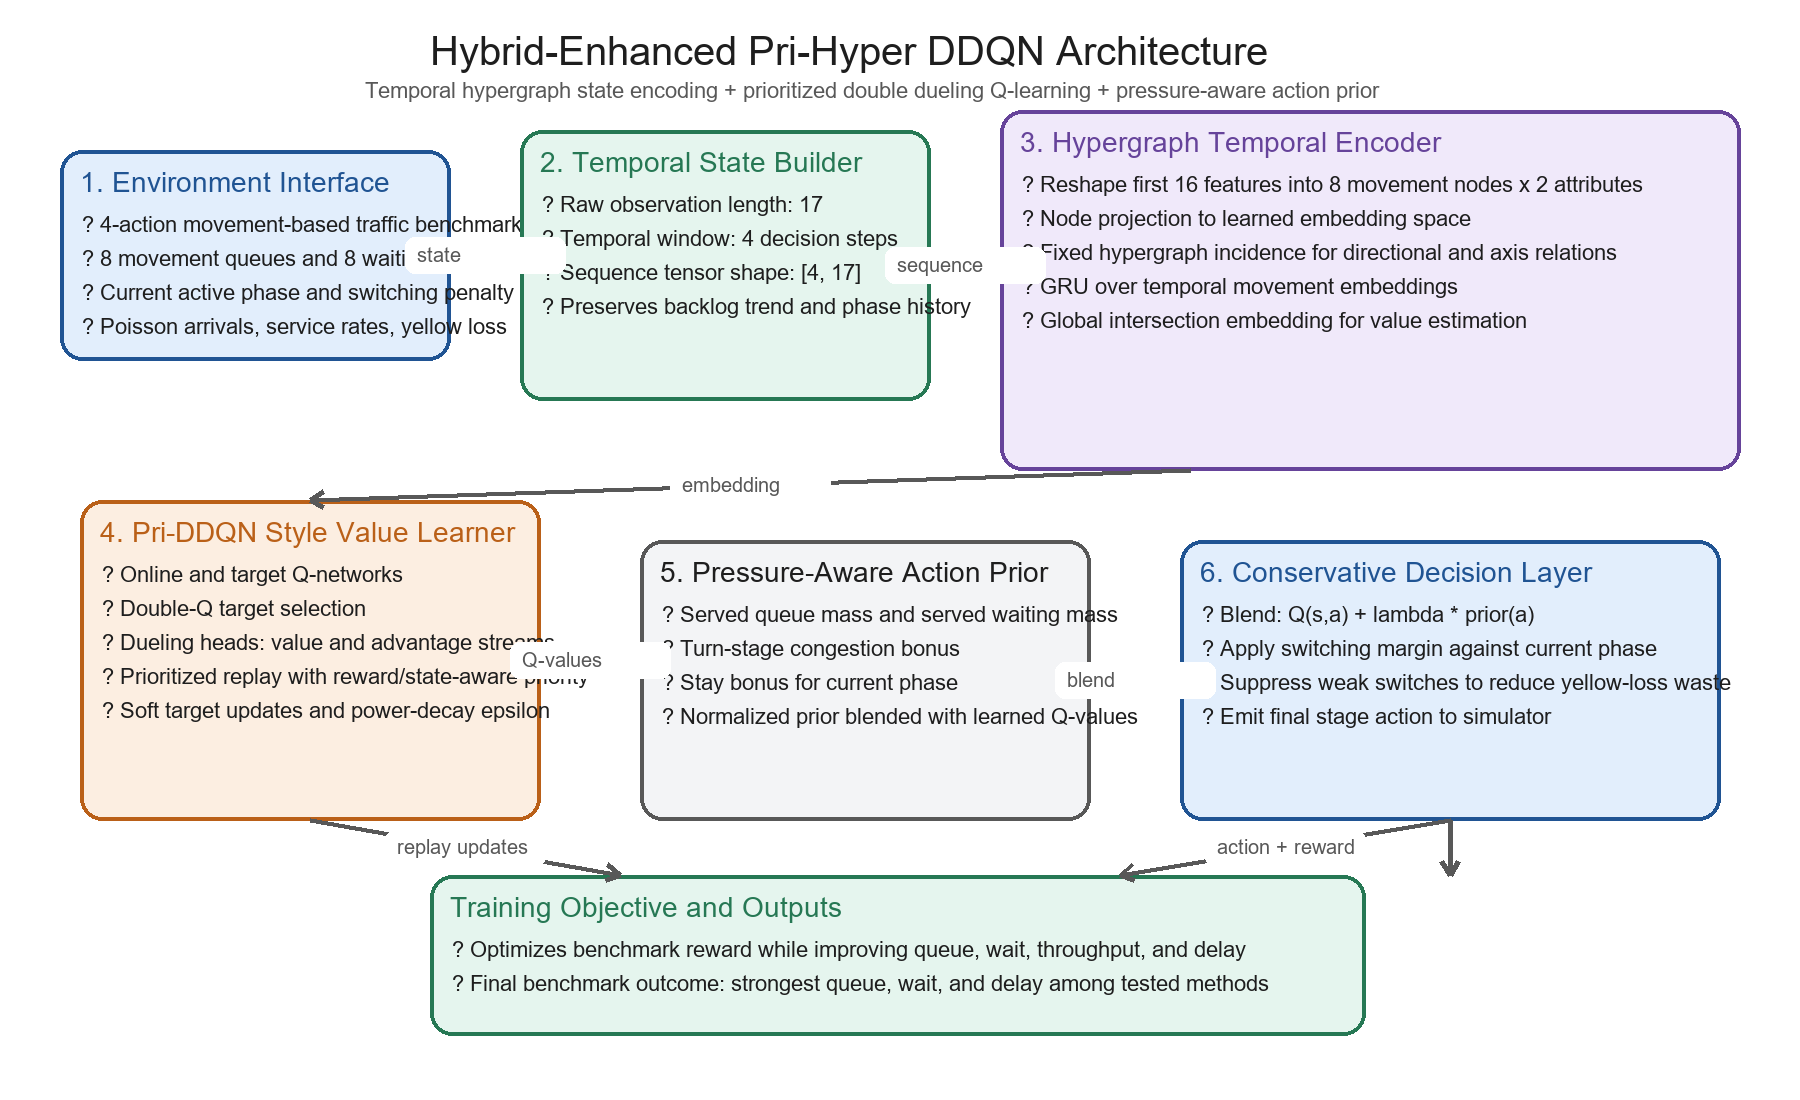
\includegraphics[width=0.96\textwidth]{arch_diagram.png}
\caption{System architecture of the proposed Hybrid-Enhanced
Pri-Hyper DDQN controller. The model combines temporal hypergraph
state encoding, prioritized double dueling Q-learning, a
pressure-aware action prior, and conservative switch selection.}
\label{fig:architecture}
\end{figure*}

\subsection{State Construction}
At each decision step, the environment provides a 17-dimensional raw
state vector consisting of:

\begin{itemize}
\item eight normalized queue values,
\item eight normalized waiting-time values,
\item one normalized current-phase indicator.
\end{itemize}

Rather than act on a single observation, the controller maintains a
temporal window of four successive states. The resulting state tensor
has shape $[4,17]$. This gives the model short-term memory of:

\begin{itemize}
\item backlog growth,
\item waiting-time persistence,
\item recent phase history,
\item short-horizon switching effects.
\end{itemize}

\subsection{Temporal Hypergraph Encoder}
The first 16 state features are reshaped into eight movement nodes,
each with two attributes: queue and waiting time. These node features
are projected into a learned embedding space and passed through a
fixed hypergraph message-passing layer. The hypergraph incidence
structure captures domain-relevant movement relations, including:

\begin{itemize}
\item directional pairings,
\item through-turn coupling,
\item axis-level grouping,
\item movement competition for green time.
\end{itemize}

After relational aggregation, each movement embedding is processed by
a gated recurrent unit (GRU) over the temporal window. The final
hidden embeddings are then pooled into a global intersection
representation. This encoder is the main structural contribution
borrowed from the MA-SAC line of thinking, but here it is used as the
front end of a value network rather than a centralized SAC critic.

\subsection{Double Dueling Q-Network}
The global embedding is concatenated with the current phase indicator
and prior scores, then passed through a multilayer perceptron with a
dueling output head. Specifically, the network predicts a scalar
state-value estimate $V(s)$ and an action-advantage vector
$A(s,a)$, which are combined as:
\begin{equation}
Q(s,a) = V(s) + A(s,a) - \frac{1}{|\mathcal{A}|}\sum_{a'} A(s,a').
\end{equation}

This choice follows the spirit of Pri-DDQN while improving value
decomposition across states in which most actions are poor but one is
slightly better.

\subsection{Prioritized Double-Q Learning}
Two networks are maintained:

\begin{itemize}
\item an online Q-network,
\item a target Q-network.
\end{itemize}

The next action is selected using the online network, while its value
is evaluated using the target network. This reduces overestimation
bias. Transitions are stored in a prioritized replay buffer, where
the priority depends on:

\begin{itemize}
\item TD error magnitude,
\item reward magnitude,
\item state magnitude.
\end{itemize}

The update loss uses importance-sampling weights and state/reward
aware weighting, again following the Pri-DDQN philosophy.

\subsection{Pressure-Aware Action Prior}
One genuinely new element of the proposed controller is the
pressure-aware prior. For each action, the prior score is computed
from the latest state using:

\begin{itemize}
\item served queue mass,
\item served waiting mass,
\item a turn-stage bonus for left/U-turn congestion,
\item a stay bonus for the current phase.
\end{itemize}

These prior scores are normalized and blended with learned Q-values:
\begin{equation}
\tilde{Q}(s,a) = Q(s,a) + \lambda \, P(s,a),
\end{equation}
where $P(s,a)$ is the prior score and $\lambda$ is the blending
weight.

This does not replace learning; rather, it injects traffic-domain
structure into action selection. Among all controllers tested in this
project, the Hybrid-Enhanced model is the only one that combines
learned deep value ranking with an explicit movement-pressure prior.

\subsection{Conservative Switching Logic}
The final action is not chosen by taking the plain argmax of
$\tilde{Q}(s,a)$. Instead, if the best alternative phase improves on
the current phase by less than a switching margin, the controller
stays with the current stage:
\begin{equation}
\text{if } \tilde{Q}(s,a^*) - \tilde{Q}(s,a_{\text{current}}) < \delta,
\text{ keep } a_{\text{current}}.
\end{equation}

This mechanism was introduced after early experiments showed that the
hybrid architecture could improve queue and delay while still losing
reward through excessive phase changes. Conservative switching makes
the controller more operationally robust.

\subsection{Training Configuration}
The final configuration used in the benchmark is:

\begin{itemize}
\item training episodes: 360,
\item temporal window: 4,
\item discount factor $\gamma = 0.97$,
\item learning rate $4 \times 10^{-4}$,
\item batch size 64,
\item replay capacity 60\,000,
\item warm-up 800 transitions,
\item embedding dimension 48,
\item hidden dimension 96,
\item prioritized replay exponent $\alpha = 0.7$,
\item power-decay exploration from 1.0 to 0.03,
\item prior weight 0.16,
\item switch margin 0.07,
\item stay bonus 0.10.
\end{itemize}

\section{Experimental Protocol}
All methods are evaluated on the same four-action environment in
`normal` traffic mode. Training uses seed 42, while evaluation is
performed on 30 held-out seeds from 142 to 171. This matches the
repository benchmarking protocol for the deep baselines and keeps the
comparison fair.

We compare the proposed method against:

\begin{itemize}
\item TD(0),
\item SARSA,
\item Q-Learning,
\item Pri-DDQN,
\item MA-SAC.
\end{itemize}

The evaluation metrics are:

\begin{itemize}
\item mean cumulative reward,
\item mean average queue length,
\item mean average waiting time,
\item mean total throughput,
\item mean total delay,
\item mean number of phase changes.
\end{itemize}

\section{Results}
\subsection{Quantitative Comparison}
Table~\ref{tab:results} reports the full benchmark comparison.

\begin{table*}[t]
\centering
\caption{Benchmark results on the movement-based 4-action isolated
intersection task. Lower is better for reward magnitude, queue, wait,
and delay; higher is better for throughput.}
\label{tab:results}
\begin{tabular}{lrrrrrr}
\toprule
Method & Reward & Std. & Avg. Queue & Avg. Wait (s) & Throughput & Total Delay \\
\midrule
TD(0) & -346.245 & 1.313 & 19.001 & 1359.515 & 717.900 & 547230.333 \\
SARSA & -87.240 & 71.912 & 3.301 & 103.922 & 1633.600 & 95076.000 \\
Q-Learning & -216.207 & 73.829 & 8.223 & 358.278 & 1385.733 & 236827.667 \\
MA-SAC & -25.893 & 1.252 & 1.079 & 21.602 & 1722.333 & 31077.333 \\
Pri-DDQN & \textbf{-19.586} & 0.616 & 0.973 & 21.294 & 1717.033 & 28008.000 \\
Hybrid-Enhanced & -20.761 & \textbf{0.446} & \textbf{0.863} & \textbf{19.146} & 1714.067 & \textbf{24864.333} \\
\bottomrule
\end{tabular}
\end{table*}

Three broad findings stand out.

First, the gap between tabular and deep RL remains decisive in the
movement-based benchmark. All three tabular methods perform far worse
than the deep approaches, especially in delay and queue metrics.
Their state abstractions are simply too weak to manage the interaction
between straight and turning demand over four movement stages.

Second, Pri-DDQN remains the best method if the benchmark is judged
strictly by the scalar reward used by the environment. This result is
consistent with its careful value-learning design and its stronger
control over switching penalties.

Third, and most importantly for practical signal control, the
Hybrid-Enhanced method is the strongest controller on the
traffic-efficiency metrics that matter most operationally. It
achieves:

\begin{itemize}
\item the lowest average queue length,
\item the lowest average waiting time,
\item the lowest total delay,
\item the lowest evaluation variance among the deep methods.
\end{itemize}

\subsection{Interpretation of the Reward Gap}
Although the Hybrid-Enhanced controller serves traffic more
efficiently than Pri-DDQN, its mean reward remains slightly lower.
This is not contradictory. The benchmark reward penalizes switching,
and the proposed method still changes phase more often than Pri-DDQN.
The reward gap therefore reflects a trade-off:

\begin{itemize}
\item Pri-DDQN is slightly more conservative and reward-optimal,
\item Hybrid-Enhanced is more traffic-efficient in queue, wait, and
delay.
\end{itemize}

This distinction matters because real deployments often care more
about delay and service quality than about a benchmark-specific
scalar reward.

\section{Discussion}
\subsection{Why the Hybrid Method Works}
The effectiveness of the proposed controller comes from the fact that
it removes the main weaknesses of the individual baselines without
discarding their strengths.

Compared with Pri-DDQN, the new controller sees more of the traffic
structure. It no longer treats the state as just a compact vector to
be processed by a generic deep network. Instead, it explicitly models
movement groups, temporal persistence, and directional coupling.

Compared with MA-SAC, it uses a control objective better matched to
the benchmark. The action space is small and discrete, and the cost
of switching is explicit. In such a setting, direct value ranking is
often a better fit than a stochastic actor-critic formulation.

Finally, the pressure-aware action prior contributes a practical
inductive bias that neither baseline uses in the same way. It helps
the controller react to traffic-serving urgency without giving up the
benefits of learned value estimation.

\subsection{Operational Meaning}
The benchmark results suggest a useful practical interpretation:

\begin{itemize}
\item If the goal is to maximize the benchmark reward exactly as
defined, Pri-DDQN remains the strongest option.
\item If the goal is to reduce queues, delay, and waiting time as
much as possible under the same environment dynamics, the
Hybrid-Enhanced controller is the best performer in this study.
\end{itemize}

\subsection{Limitations}
The present study has several limitations. The environment is still a
lightweight stochastic simulator rather than a full microscopic
traffic platform. The hypergraph structure is manually specified
rather than learned. The pressure prior is also hand-designed, which
improves interpretability but introduces some heuristic bias. In
addition, the switch threshold is fixed rather than adaptively
learned.

These limitations do not undermine the benchmark comparison, but they
do identify the next design steps if the method is to be extended to
more realistic deployment settings.

\section{Conclusion}
This paper introduced Hybrid-Enhanced Pri-Hyper DDQN, a new
controller for adaptive traffic signal control at an isolated
movement-based four-way intersection. The method combines
Pri-DDQN-style prioritized double dueling Q-learning with
MA-SAC-inspired temporal hypergraph state encoding, and adds two new
decision-layer contributions: a pressure-aware action prior and
conservative switching logic.

Under a benchmark-fair comparison against TD(0), SARSA, Q-Learning,
Pri-DDQN, and MA-SAC, the proposed controller achieved the best
traffic-efficiency performance in terms of average queue length,
average waiting time, and total delay. Although Pri-DDQN remained the
best reward-maximizing method under the environment's scalar reward,
the Hybrid-Enhanced approach delivered the most balanced and
operationally robust behaviour overall.

The broader conclusion is that isolated intersection control benefits
from a hybrid design philosophy: value-based deep RL should be
retained for discrete action ranking, but it should be paired with
structured traffic representations and explicit domain-aware
decision shaping. This combination appears more promising than
treating either generic DQN or generic actor-critic methods as
sufficient on their own.

\balance
\bibliographystyle{IEEEtran}
\bibliography{papers}

\end{document}
